


\tikzset{every picture/.style={line width=1.05pt}} %set default line width to 0.75pt        

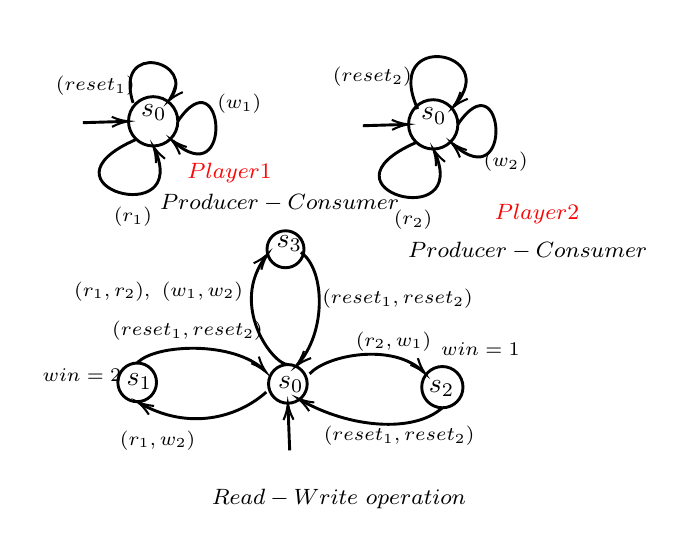
\begin{tikzpicture}[x=0.55pt,y=0.55pt,yscale=-1,xscale=1]
%uncomment if require: \path (0,300); %set diagram left start at 0, and has height of 300

%Shape: Circle [id:dp8314413576675287] 
\draw   (149.6,126.85) .. controls (149.6,120.14) and (155.04,114.7) .. (161.75,114.7) .. controls (168.46,114.7) and (173.9,120.14) .. (173.9,126.85) .. controls (173.9,133.56) and (168.46,139) .. (161.75,139) .. controls (155.04,139) and (149.6,133.56) .. (149.6,126.85) -- cycle ;
%Shape: Circle [id:dp7772472429687135] 
\draw   (150.6,215.3) .. controls (150.6,208.29) and (156.29,202.6) .. (163.3,202.6) .. controls (170.31,202.6) and (176,208.29) .. (176,215.3) .. controls (176,222.31) and (170.31,228) .. (163.3,228) .. controls (156.29,228) and (150.6,222.31) .. (150.6,215.3) -- cycle ;
%Shape: Circle [id:dp8090258776189614] 
\draw   (251.25,217.45) .. controls (251.25,209.97) and (257.32,203.9) .. (264.8,203.9) .. controls (272.28,203.9) and (278.35,209.97) .. (278.35,217.45) .. controls (278.35,224.93) and (272.28,231) .. (264.8,231) .. controls (257.32,231) and (251.25,224.93) .. (251.25,217.45) -- cycle ;
%Shape: Circle [id:dp44457702069517324] 
\draw   (51.6,214.3) .. controls (51.6,207.29) and (57.29,201.6) .. (64.3,201.6) .. controls (71.31,201.6) and (77,207.29) .. (77,214.3) .. controls (77,221.31) and (71.31,227) .. (64.3,227) .. controls (57.29,227) and (51.6,221.31) .. (51.6,214.3) -- cycle ;
%Curve Lines [id:da7159034648648847] 
\draw    (163.3,202.6) .. controls (153.45,202.6) and (124.2,163.79) .. (149.12,131.19) ;
\draw [shift={(150.3,129.7)}, rotate = 129.37] [color={rgb, 255:red, 0; green, 0; blue, 0 }  ][line width=0.75]    (10.93,-3.29) .. controls (6.95,-1.4) and (3.31,-0.3) .. (0,0) .. controls (3.31,0.3) and (6.95,1.4) .. (10.93,3.29)   ;
%Curve Lines [id:da856509401174204] 
\draw    (171.9,128.85) .. controls (188.17,140.51) and (188.49,182.04) .. (169.68,202.52) ;
\draw [shift={(168.5,203.75)}, rotate = 315] [color={rgb, 255:red, 0; green, 0; blue, 0 }  ][line width=0.75]    (10.93,-3.29) .. controls (6.95,-1.4) and (3.31,-0.3) .. (0,0) .. controls (3.31,0.3) and (6.95,1.4) .. (10.93,3.29)   ;
%Curve Lines [id:da5490799952546435] 
\draw    (149.1,220.7) .. controls (130.39,237.44) and (98.09,246.43) .. (65.78,227.87) ;
\draw [shift={(64.3,227)}, rotate = 30.99] [color={rgb, 255:red, 0; green, 0; blue, 0 }  ][line width=0.75]    (10.93,-3.29) .. controls (6.95,-1.4) and (3.31,-0.3) .. (0,0) .. controls (3.31,0.3) and (6.95,1.4) .. (10.93,3.29)   ;
%Curve Lines [id:da32420249193131656] 
\draw    (64.3,201.6) .. controls (75.86,188.96) and (127.96,186.78) .. (147.92,206.47) ;
\draw [shift={(149.1,207.7)}, rotate = 227.86] [color={rgb, 255:red, 0; green, 0; blue, 0 }  ][line width=0.75]    (10.93,-3.29) .. controls (6.95,-1.4) and (3.31,-0.3) .. (0,0) .. controls (3.31,0.3) and (6.95,1.4) .. (10.93,3.29)   ;
%Curve Lines [id:da5468630552582512] 
\draw    (177.6,208.7) .. controls (189.16,196.06) and (232.81,188.03) .. (252.43,207.47) ;
\draw [shift={(253.6,208.7)}, rotate = 227.86] [color={rgb, 255:red, 0; green, 0; blue, 0 }  ][line width=0.75]    (10.93,-3.29) .. controls (6.95,-1.4) and (3.31,-0.3) .. (0,0) .. controls (3.31,0.3) and (6.95,1.4) .. (10.93,3.29)   ;
%Curve Lines [id:da7774551676749778] 
\draw    (264.8,231) .. controls (246.09,247.75) and (203.7,244.5) .. (171.08,225.58) ;
\draw [shift={(169.6,224.7)}, rotate = 30.99] [color={rgb, 255:red, 0; green, 0; blue, 0 }  ][line width=0.75]    (10.93,-3.29) .. controls (6.95,-1.4) and (3.31,-0.3) .. (0,0) .. controls (3.31,0.3) and (6.95,1.4) .. (10.93,3.29)   ;
%Straight Lines [id:da9977682076817751] 
\draw    (164.5,259) -- (163.38,230) ;
\draw [shift={(163.3,228)}, rotate = 87.78] [color={rgb, 255:red, 0; green, 0; blue, 0 }  ][line width=0.75]    (10.93,-3.29) .. controls (6.95,-1.4) and (3.31,-0.3) .. (0,0) .. controls (3.31,0.3) and (6.95,1.4) .. (10.93,3.29)   ;
%Shape: Circle [id:dp1467498401619306] 
\draw   (242.6,44.8) .. controls (242.6,35.85) and (249.85,28.6) .. (258.8,28.6) .. controls (267.75,28.6) and (275,35.85) .. (275,44.8) .. controls (275,53.75) and (267.75,61) .. (258.8,61) .. controls (249.85,61) and (242.6,53.75) .. (242.6,44.8) -- cycle ;

%Curve Lines [id:da20144538683966495] 
\draw    (248.6,34.7) .. controls (224.84,-17.77) and (304.97,-3.59) .. (272.62,32.6) ;
\draw [shift={(271.6,33.7)}, rotate = 313.41] [color={rgb, 255:red, 0; green, 0; blue, 0 }  ][line width=0.75]    (10.93,-3.29) .. controls (6.95,-1.4) and (3.31,-0.3) .. (0,0) .. controls (3.31,0.3) and (6.95,1.4) .. (10.93,3.29)   ;
%Curve Lines [id:da01826233197981253] 
\draw    (275,44.8) .. controls (305.29,0.15) and (312.46,93.79) .. (271.85,57.83) ;
\draw [shift={(270.6,56.7)}, rotate = 42.88] [color={rgb, 255:red, 0; green, 0; blue, 0 }  ][line width=0.75]    (10.93,-3.29) .. controls (6.95,-1.4) and (3.31,-0.3) .. (0,0) .. controls (3.31,0.3) and (6.95,1.4) .. (10.93,3.29)   ;
%Curve Lines [id:da45337553182486945] 
\draw    (247.6,56.7) .. controls (177.31,87.39) and (284.42,117.1) .. (259.59,62.68) ;
\draw [shift={(258.8,61)}, rotate = 63.88] [color={rgb, 255:red, 0; green, 0; blue, 0 }  ][line width=0.75]    (10.93,-3.29) .. controls (6.95,-1.4) and (3.31,-0.3) .. (0,0) .. controls (3.31,0.3) and (6.95,1.4) .. (10.93,3.29)   ;
%Straight Lines [id:da9810106035384246] 
\draw    (212.6,45.7) -- (240.6,44.86) ;
\draw [shift={(242.6,44.8)}, rotate = 178.28] [color={rgb, 255:red, 0; green, 0; blue, 0 }  ][line width=0.75]    (10.93,-3.29) .. controls (6.95,-1.4) and (3.31,-0.3) .. (0,0) .. controls (3.31,0.3) and (6.95,1.4) .. (10.93,3.29)   ;
%Shape: Circle [id:dp6710432398464078] 
\draw   (58.6,42.8) .. controls (58.6,33.85) and (65.85,26.6) .. (74.8,26.6) .. controls (83.75,26.6) and (91,33.85) .. (91,42.8) .. controls (91,51.75) and (83.75,59) .. (74.8,59) .. controls (65.85,59) and (58.6,51.75) .. (58.6,42.8) -- cycle ;

%Curve Lines [id:da7849548233918409] 
\draw    (61.6,30.7) .. controls (48.27,-11.15) and (104.67,3.38) .. (85.85,28.17) ;
\draw [shift={(84.6,29.7)}, rotate = 311.08] [color={rgb, 255:red, 0; green, 0; blue, 0 }  ][line width=0.75]    (10.93,-3.29) .. controls (6.95,-1.4) and (3.31,-0.3) .. (0,0) .. controls (3.31,0.3) and (6.95,1.4) .. (10.93,3.29)   ;
%Curve Lines [id:da3143750611128635] 
\draw    (91,42.8) .. controls (121.29,-1.85) and (128.46,91.79) .. (87.85,55.83) ;
\draw [shift={(86.6,54.7)}, rotate = 42.88] [color={rgb, 255:red, 0; green, 0; blue, 0 }  ][line width=0.75]    (10.93,-3.29) .. controls (6.95,-1.4) and (3.31,-0.3) .. (0,0) .. controls (3.31,0.3) and (6.95,1.4) .. (10.93,3.29)   ;
%Curve Lines [id:da830110688853805] 
\draw    (63.6,54.7) .. controls (-6.69,85.39) and (100.42,115.1) .. (75.59,60.68) ;
\draw [shift={(74.8,59)}, rotate = 63.88] [color={rgb, 255:red, 0; green, 0; blue, 0 }  ][line width=0.75]    (10.93,-3.29) .. controls (6.95,-1.4) and (3.31,-0.3) .. (0,0) .. controls (3.31,0.3) and (6.95,1.4) .. (10.93,3.29)   ;
%Straight Lines [id:da9076150365855119] 
\draw    (28.6,43.7) -- (56.6,42.86) ;
\draw [shift={(58.6,42.8)}, rotate = 178.28] [color={rgb, 255:red, 0; green, 0; blue, 0 }  ][line width=0.75]    (10.93,-3.29) .. controls (6.95,-1.4) and (3.31,-0.3) .. (0,0) .. controls (3.31,0.3) and (6.95,1.4) .. (10.93,3.29)   ;


% Text Node
\draw (297,95) node [anchor=north west][inner sep=0.75pt]  [font=\footnotesize,color={rgb, 255:red, 247; green, 6; blue, 6 }  ,opacity=1 ]  {$Player2$};
% Text Node
\draw (77,88) node [anchor=north west][inner sep=0.75pt]  [font=\footnotesize]  {$Producer-Consumer$};
% Text Node
\draw (8.6,10.7) node [anchor=north west][inner sep=0.75pt]  [font=\scriptsize]  {$( reset_{1})$};
% Text Node
\draw (114.6,22.7) node [anchor=north west][inner sep=0.75pt]  [font=\scriptsize]  {$( w_{1})$};
% Text Node
\draw (46.6,96.7) node [anchor=north west][inner sep=0.75pt]  [font=\scriptsize]  {$( r_{1})$};
% Text Node
\draw (95,68) node [anchor=north west][inner sep=0.75pt]  [font=\footnotesize,color={rgb, 255:red, 252; green, 6; blue, 6 }  ,opacity=1 ]  {$Player1$};
% Text Node
\draw (240,120) node [anchor=north west][inner sep=0.75pt]  [font=\footnotesize]  {$Producer-Consumer$};
% Text Node
\draw (190.6,4.7) node [anchor=north west][inner sep=0.75pt]  [font=\scriptsize]  {$( reset_{2})$};
% Text Node
\draw (289.6,60.7) node [anchor=north west][inner sep=0.75pt]  [font=\scriptsize]  {$( w_{2})$};
% Text Node
\draw (230.6,98.7) node [anchor=north west][inner sep=0.75pt]  [font=\scriptsize]  {$( r_{2})$};
% Text Node
\draw (111,282) node [anchor=north west][inner sep=0.75pt]  [font=\footnotesize]  {$Read-Write\ operation$};
% Text Node
\draw (-0.2,202.7) node [anchor=north west][inner sep=0.75pt]  [font=\scriptsize]  {$win=2$};
% Text Node
\draw (261.6,185.7) node [anchor=north west][inner sep=0.75pt]  [font=\scriptsize]  {$win=1$};
% Text Node
\draw (45.6,171.7) node [anchor=north west][inner sep=0.75pt]  [font=\scriptsize]  {$( reset_{1} ,reset_{2})$};
% Text Node
\draw (184.6,240.7) node [anchor=north west][inner sep=0.75pt]  [font=\scriptsize]  {$( reset_{1} ,reset_{2})$};
% Text Node
\draw (205.6,178.7) node [anchor=north west][inner sep=0.75pt]  [font=\scriptsize]  {$( r_{2} ,w_{1})$};
% Text Node
\draw (50.6,243.7) node [anchor=north west][inner sep=0.75pt]  [font=\scriptsize]  {$( r_{1} ,w_{2})$};
% Text Node
\draw (20.6,145.7) node [anchor=north west][inner sep=0.75pt]  [font=\scriptsize]  {$( r_{1} ,r_{2}) ,\ ( w_{1} ,w_{2})$};
% Text Node
\draw (183.6,150.7) node [anchor=north west][inner sep=0.75pt]  [font=\scriptsize]  {$( reset_{1} ,reset_{2})$};
% Text Node
\draw (153.6,115.7) node [anchor=north west][inner sep=0.75pt]    {$s_{3}$};
% Text Node
\draw (253.6,210.7) node [anchor=north west][inner sep=0.75pt]    {$s_{2}$};
% Text Node
\draw (154.6,208) node [anchor=north west][inner sep=0.75pt]    {$s_{0}$};
% Text Node
\draw (55,206) node [anchor=north west][inner sep=0.75pt]    {$s_{1}$};
% Text Node
\draw (64.6,29.7) node [anchor=north west][inner sep=0.75pt]    {$s_{0}$};
% Text Node
\draw (248.6,31.7) node [anchor=north west][inner sep=0.75pt]    {$s_{0}$};


\end{tikzpicture}
